\documentclass[a4paper, 12pt]{article}%тип документа

%отступы
\usepackage[left=2cm,right=2cm,top=2cm,bottom=3cm,bindingoffset=0cm]{geometry}

%Русский язык
\usepackage[T2A]{fontenc} %кодировка
\usepackage[utf8]{inputenc} %кодировка исходного кода
\usepackage[english,russian]{babel} %локализация и переносы

%Вставка картинок
\usepackage{wrapfig}
\usepackage{graphicx}
\graphicspath{{pictures/}}
\DeclareGraphicsExtensions{.pdf,.png,.jpg}

%оглавление
\usepackage{titlesec}
\titlespacing{\chapter}{0pt}{-30pt}{12pt}
\titlespacing{\section}{\parindent}{5mm}{5mm}
\titlespacing{\subsection}{\parindent}{5mm}{5mm}
\usepackage{setspace}

%Графики
\usepackage{multirow}
\usepackage{pgfplots}
\pgfplotsset{compat=1.9}

%Математика
\usepackage{amsmath, amsfonts, amssymb, amsthm, mathtools}

%Стиль страницы
\usepackage{fancyhdr}
\pagestyle{fancy}

\begin{document}

\begin{titlepage}

\begin{center}
%\vspace*{1cm}
\large\textbf{Московский Физико-Технический Институт}\\
\large\textbf{(государственный университет)}
\vfill
\line(1,0){430}\\[1mm]
\huge\textbf{Работа 4.7.1.}\\
\line(1,0){430}\\[1mm]
\vfill
\large Сибгатуллин Булат, ФРКТ\\
\end{center}

\end{titlepage}
\fancyhead[L] {Работа 4.7.1.}
\noindent \textbf{Цель работы:} \\
\indent изучение зависимости показателя преломления необыкновенной волны от направления в двоякопреломляющем кристалле; определение главных показателей преломления $n_\text{о}$ и $n_\text{е}$ -- необыкновенной волны в кристалле; наблюдение эффекта полного отражения.\\
\noindent \textbf{В работе используются:} \\
\indent гелий-неновый лазер, вращающийся столик с неподвижным лимбом, призма из исландского шпата, поляроид.

\section*{Описание работы}

При падении световой волны на границу изотропной среды в этой
среде от границы распространяется одна волна. Если среда анизотропна, то в ней в общем случае возникают две волны, распространяющиеся
от границы в разных направлениях и с разными скоростями. Это явление называется \textit{двойным лучепреломлением}.

\textbf{Плаские волны в кристаллах.} В кристаллических средах в отсутствие электрических зарядов и токо справделивы уравнения Максвелла:

\begin{equation}
rot \overrightarrow{H} = \frac{1}{c}\frac{\partial \overrightarrow{D}}{\partial t}, \quad rot \overrightarrow{E} = - \frac{1}{c} \frac{\partial \overrightarrow{B}}{\partial t}
\end{equation}

Если среды прозрачны и однородны, то в них могут распространяться плоские монохроматические волны. Запишем такую волну в комплексном виде:

\[\overrightarrow{E} = \overrightarrow{E}_0 e^{i(\omega t - \overrightarrow{k}\overrightarrow{r}}); \quad
\overrightarrow{B} = \overrightarrow{H} = \overrightarrow{H}_0 e^{i(\omega t - \overrightarrow{k}\overrightarrow{r}}); \quad
\overrightarrow{D} = \overrightarrow{D}_0 e^{i(\omega t - \overrightarrow{k}\overrightarrow{r}}\]

Тогда уравнения (1) можем записать в виде:

\[rot \overrightarrow{H} = -i [\overrightarrow{k} \overrightarrow{H}]\]

и аналогично для $rot \overrightarrow{E}$. В результате (1) перейдут в

\[[\overrightarrow{k} \overrightarrow{H}] = -\frac{\omega}{c} \overrightarrow{D}; \quad [\overrightarrow{k} \overrightarrow{E}] = \frac{\omega}{c} \overrightarrow{D}\]

Для характеристики оптических свойств анизотропной среды требуется девять величин $\varepsilon_{ij}$, образующих тензор диэлектрической проницаемости. Он вводится посредством соотношени:

\begin{equation}
D_i = \sum\limits_j \varepsilon_{ij} E_j \quad (i,j = x,y,z).
\end{equation}

Благодаря тензорной связи между $\overrightarrow{D}$ и $\overrightarrow{E}$ направления этих векторов в кристаллах. Зададим за $\overrightarrow{S} = \frac{c}{4\pi} \left[ \overrightarrow{E} \overrightarrow{H} \right]$ вектор Пойнтинга. Четыре вектора $\overrightarrow{D}, \overrightarrow{E}, \overrightarrow{N}, \overrightarrow{S}$ лежат в одной плоскости, перпендикулярной вектору $\overrightarrow{H}$.

 \textbf{Оптически одноосные кристаллы.} Всю совокупность возможных значений тензора диэлектрической проницаемости можно представить при помощи трехосного эллипсоида. Значение диэлектрической проницаемости для любого направления выражается длиной радиуса-вектора эллипсоида, проведенного по этому направлению. Три значения диэлектричеcкой проницаемости $\varepsilon_x, \varepsilon_y, \varepsilon_z$, соответствующие осям эллипсоидв, называются \textit{главными значениями диэлектрической проницаемости} и соответственно $\sqrt{\varepsilon_x}, \sqrt{\varepsilon_y}, \sqrt{\varepsilon_z}$ --- \textit{главными показателями преломления}.

В системе координат, оси которой совпадают с главными осями эллипсоида, тензор диэлектрической проницаемости приводится к диагональному виду, и проекции векторов $D$ и $E$ на оси координат связаны простыми соотношениями:
\begin{equation*}
	D_x = \varepsilon_x E_x, \quad D_y = \varepsilon_y E_y, \quad D_z = \varepsilon_z E_z.
\end{equation*}

В оптически одноосном кристалле, каковым является исландский шпат, эллипсоид диэлектрической проницаемости представляет собой эллипсоид вращения.
В нём оптическая ось совпадает с осью вращения эллипсоида диэлектрических проницаемостей. Для главных значений диэлектрических проницаемостей приняты обозначения $\varepsilon_z = \varepsilon_\parallel$ и $\varepsilon_x = \varepsilon_y = \varepsilon_\perp$. В дальнейшем нам потребуется связь между проекциями векторов $\vec D$ и $\vec E$ на оптическую ось кристалла $(\vec D_\parallel $ и $\vec E_\parallel )$ и на плоскость, перпендикулярную оси $(\vec D_\perp $ и $\vec E_\perp )$:
\begin{equation}
	\vec D_\parallel  = \varepsilon_\parallel \vec E_\parallel , \quad \vec D_\perp  = \varepsilon_\perp \vec E_\perp. 
\end{equation}

\begin{wrapfigure}{r}{0.45\textwidth}
    \centering
    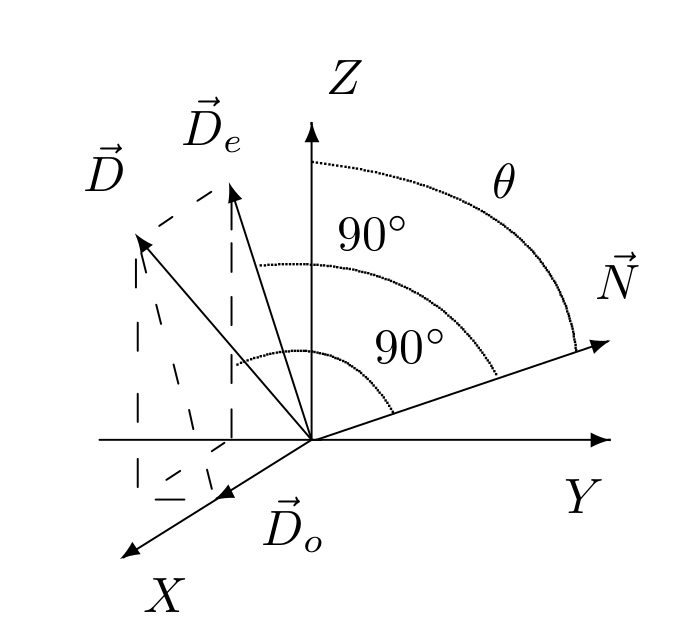
\includegraphics[width=0.5\textwidth]{images/DN.png}
    \caption{Расположение векторов $\vec N$ и $\vec D$ в анизотропной среде: $(\vec D = \vec D_o + \vec D_e; \vec D_o \perp \vec D_e; \vec D \perp \vec N);$ $\vec N$ и $\vec D_e$ лежат в плоскости $(Z, Y)$; $\vec D_o$ перпендикулярен плоскости $(Z, Y)$}
\end{wrapfigure} 
Волну, распространяющуюся в одноосном кристалле, можно разделить на две линейно поляризованные волны: обыкновенную, вектор электрической индукции $\vec D_o$ которой перпендикулярен главному сеению, и необыкновенную, с вектором электрической индукции $\vec D_e$, лежащим в главном сечении (рис. 2) \textit{Главным сечением кристалла} называется плоскость, в которой лежит оптическая ось кристалла и нормаль к фронту волны.

Рассмотрим вначале обыкновенную волну, которой вектор $\vec D_o$ перпендикулярен главному сечению. Тогда $D_{oz} = 0$, и из условия $D_z = \varepsilon_z E_z$ следует, что $E_{oz} = 0.$ Кроме того, так как $D_{oy} = \varepsilon_\perp E_{oy}$ и $D_{ox} = \varepsilon_\perp E_{ox}$, то можно записать 
\begin{equation}
	\vec D_o = \varepsilon_\perp \vec E_o.
\end{equation}

Таким образом, для обыкновенной волны материальное уравнение
имеет такой же вид, как и в изотропной среде. Найдем с помощью этого
уравнения скорость распространения обыкновенной волны и соответ-
ствующий показатель преломления. Из (2) имеем
\[
	D_o = \frac{c}{v_o} H_o, \quad H_o = \frac{c}{v_o} E_o
\]
или, учитывая (5),
\[
	\varepsilon_{\perp} E_o = \frac{c}{v_o} H_o, \quad H_o = \frac{c}{v_o} E_o,
\]
откуда
\[
	v_o = \frac{c}{ \sqrt{\varepsilon_{\perp}}} \quad \text{и} \quad n_o = \frac{c}{v_o} = \sqrt{\varepsilon_\perp}.
\]
Таким образом, скорость распространения обыкновенной волны и ее показатель преломления не зависят от направления распространения.

У необыкновенной волны вектор $\vec D_e$ не параллелен $\vec E_e$, и связь между ними сложнее, чем в (5).

Для того чтобы найти скорость распространения $v$ и показатель преломления нобыкновенной волны $n = c / v$, достаточно найти связь между вектором электрической индукции этой волны $\vec D_e$ и проекцией на него вектора электрического поля волны $E_{eD}$. Тогда, подставляя $D_e = \varepsilon E_{eD}$ в (2), приходим к соотношения
\[
	\varepsilon E_{eD} = \frac{c}{v} H_e; \quad H_e = \frac{c}{v} E_{eD},
\]
формально тождественным с соотношениями для обыкновенной волны. Роль величины $\varepsilon_\perp$ тперь играет величина $\varepsilon$, а показатель преломления необыкновеной волны равен $\sqrt{\varepsilon}$.

Найдём связь между $D_e$ и $E_{eD}$. Для этого разложим векторы $\vec D_e$ и $\vec E_e$ на составляющие, параллельные и перпендикулярные оси кристалла:
\[
	\vec D_e = \vec D_{e \parallel} + \vec D_{e \perp}.
\]
\[
	\vec E_e = \vec E_{e \parallel} + \vec E_{e \perp}.
\]
Учитывая (4), находим
\[
	E_{eD} = \frac{\vec E_e \vec D_e}{D_e} = \frac{E_{e \parallel} D_{e \parallel} + E_{e \perp} D_{e \perp}}{D_e} = \frac{D^2_{e \parallel} / \varepsilon_\parallel + D^2_{e \perp} / \varepsilon_\perp}{D_e}
\]
или 
\[
E_{eD} = D_e \left( \frac{\sin^2{\theta}}{\varepsilon_\parallel} + \frac{\cos^2{\theta}}{\varepsilon_\perp} \right) = \frac{D_e}{\varepsilon},
\]
где $\theta$ "--- угол между оптической осью $Z$ и волновой нормалью $N$:
\begin{equation}
	\sin \theta = \frac{D_{e \parallel}}{D_e}, \quad \cos \theta = \frac{D_{e \perp}}{D_e}.
\end{equation}
Таким образом, $\varepsilon$ и соответственно скорость распространения и показатель преломления необыкновенной волны зависят от угла между оптической осью кристалла и   направлением распространения волны.

Выпишем выражение для показателя преломления необыкновенной волны $n = \sqrt \varepsilon$ через главные показатели преломления $n_o, n_e$ и угол $\theta$:
\begin{equation}
	\frac{1}{\left[ n(\theta) \right] ^ 2} = \frac{\sin^2 \theta}{n^2_e} + \frac{\cos^2 \theta}{n^2_o}.
\end{equation}
При $n_o - n_e \ll n_o$ и $n_e$ (для исландского шпата $n_o = 1,655, n_e = 1,485$ для $\lambda = 0,63$ мкм) (7) можно упростить:
\begin{equation}
	n(\theta) \approx n_e + (n_o - n_e) \cos^2 \theta.
\end{equation}

\noindent \textbf{Двойное лучепреломление в призме из исландского шпата.} Рассмотрим, как по преломлению лучей в кристаллической призме можно определить показатели преломления для обыкновенной и необыкновенной волны. В работе исследуется одна из двух призм, составляющих поляризатор (рис. 3).
\begin{figure}[h!]
	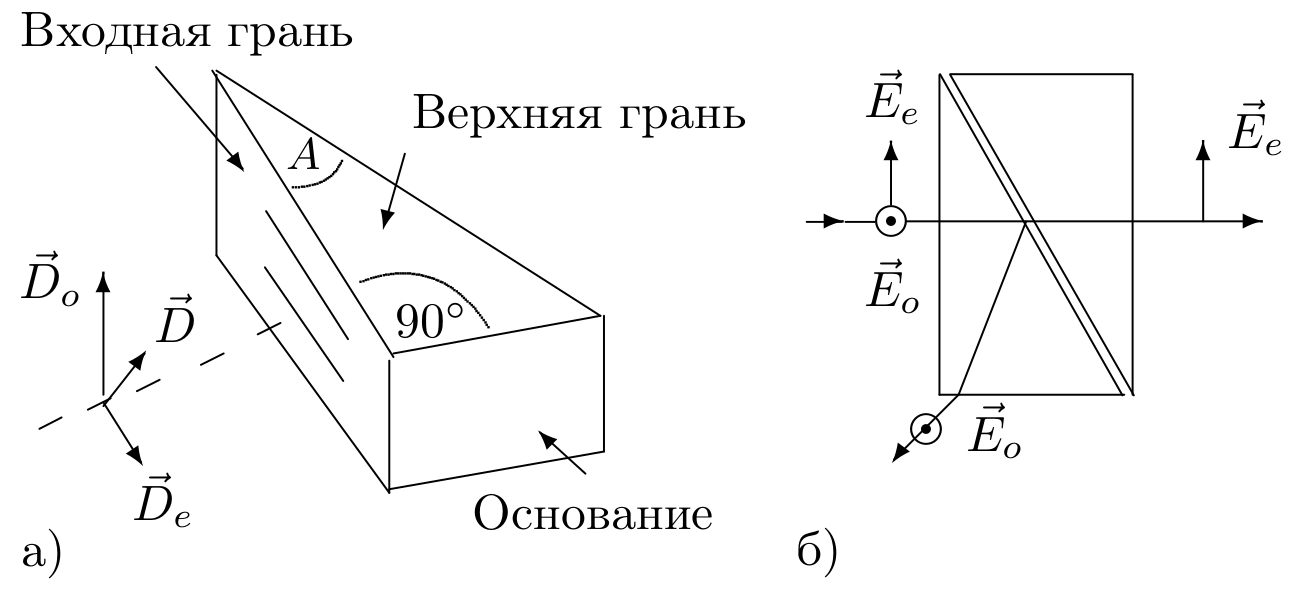
\includegraphics[width = 1.0\linewidth]{images/shpat.png}
	\caption{ а) Исследуемая призма из исландского шпата. Штриховкой указано направление оптической оси кристалла. б) Ход лучей в поляризационной призме}
\end{figure}	
В исследуемой призме ось кристалла лежит в плоскости, параллельной верхней грани призмы, причем она параллельна входной грани призмы (длинному катету). При этом в обыкновенной волне вектор $\vec D_o$ пендикулярен верхней грани призмы, а в необыкновенной волне вектор $\vec D_e$  параллелен верхней грани.
\begin{wrapfigure}{r}{0.45\textwidth}
    \centering
    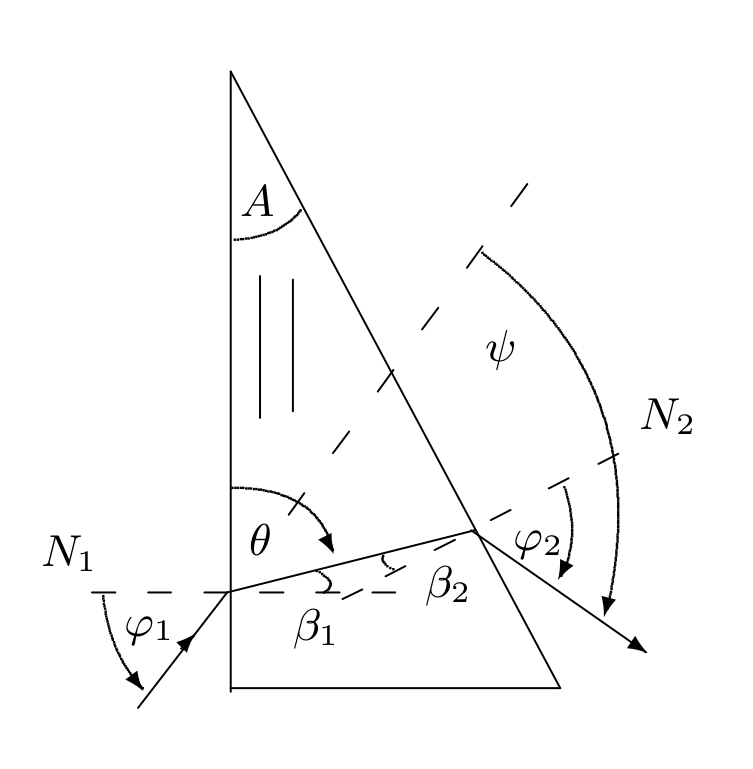
\includegraphics[width=0.5\textwidth]{images/prism.png}
    \caption{Ход лучей в призме}
\end{wrapfigure} 
Волну, падающую на входную грань призмы, можно представить в виде суммы двух ортогональных линейно поляризованных волн. Преломление этих двух волн на грани призмы можно рассматривать независимо. Волна, в которой вектор $\vec D$ направлен вертикально (перпендикулярно верхней грани и оси кристалла), внутри кристалла будет распространяться как обыкновенная. Для этой волны выполняется закон Снеллиуса, а показатель преломления призмы для нее равен $n_o$. Волна, в которой вектор $\vec D$ направлен горизонтально, в кристалле будет распространяться как необыкновенная. Для этой волны также будет выполняться закон Снеллиуса, но с тем отличием, что показатель преломления призмы для нее будет зависеть от угла между осью кристалла и волновой нормалью. 

Значение показателя преломления и угол, под которым преломилась волна в призме, можно найти, измерив угол падения на входную грань призмы $\phi_1$ и угол $\phi_2$ на выходе призмы (рис. 4). Запишем закон Снеллиуса для одной из волн применительно к первой и второй граням призмы:
\[
	\sin \phi = n \sin \beta_1;
\]
\[
	\sin \phi_2 = n \sin \beta_2 = n \sin (A - \beta_1).
\]
При этом мы выразили угол падения на вторую грань призмы $\beta_2$ через угол преломления на первой грани призмы $\beta_1$ и угол при вершине призмы $A$. Как видно из рис. 4, эти углы связаны простым соотношением $A = \beta_1 + \beta_2$. Учитывая, что угол преломления $\beta_1$ связан с углом $\theta$ между осью кристалла и волновой нормалью $\vec N$ соотношением $\theta + \beta_1 = \pi / 2$, находим $n$ и $\theta$:
\begin{equation}
n = \frac{1}{\sin A} \sqrt{\sin^2 \varphi_1 + \sin^2 \varphi_2 + 2 \sin \varphi_1 \sin \varphi_2 \cos A};
\end{equation}
\[
	\cos \theta = \frac{\sin \varphi_1}{n}.
\]
Для обыкновенной волны $n$ не будет зависеть от угла $\theta$, а для необыкновенной волны зависимость $n$ от $\theta$ должна описываться выражением (7).

Показатель преломления призмы из изотропного материала удобно находить по углу нименьшего отклонения луча от первоначального направления. Угол отклонения луча призмой ($\psi$ на рис. 4) минимален для симметричного хода лучей, то есть когда $\varphi_1 = \varphi_2$. Тогда показатель преломления можно рассчитать по формуле
\begin{equation}
n=\frac{\sin \left(\frac{\psi_{m}+A}{2}\right)}{\sin \left(\frac{A}{2}\right)},
\end{equation}
где $\psi_m$ --- угол наименьшего отклонения.

Если призма неизотропна, то этой формулой, строго говоря, можно воспользоваться только для обыкновенной волны, которая, как это было показано ранее, распространяется так же, как и в изотропной среде. Но если учесть, что угол при вершине призмы мал, и при угле наименьшего отклонения преломлённый луч в призме распространяется под углом к оси кристалла близким к $\pi / 2$, то в качестве оценки формулу (10) можно использовать для определения $n_e$.


\end{document}